\subsection{Feedforward Neural Networks (FNNs)}
Following the CNN Class with Data Augmentation, we explored Feedforward Neural Networks. This FNN approach uses Data Augmentation to techniques which are exhibited in the following image.
\begin{figure}[H]
    \centering
    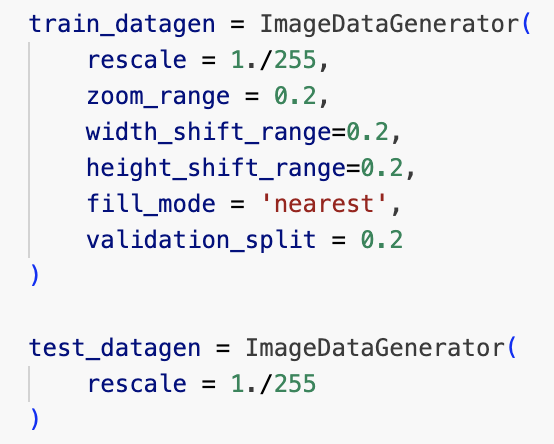
\includegraphics[width=0.5\linewidth]{images/fnn_data_aug.png}
    \caption{Data Augmentation techniques that were used.}
    \label{fig:FNN_data_aug}
\end{figure}
The techniques used include random zooms in or out on the images by up to 20\%, random shifts of the image horizontally and vertically up to 20\%, and a strategy that fills the missing pixels created by zooms and other transformations using the nearest pixel values.

The implemented FNN model includes an input layer, three hidden layers, and an output layer. As with the previous CNN, the model was compiled using the Adam optimizer and the loss function is the "categorical crossentropy".

A grid search approach of hypertuning the model was used. It consisted of trying out different values of the hyperparameters and picking the "model" that gives the best score. This approach was used for balancing computational efficiency and thoroughness in exploring hyperparameter combinations. The hyperparameters that were tuned are the number of neurons per hidden layer and the activation function of the hidden layers. The values experimented of each hyperparameter can be consulted in the table \ref{tab:fnn_hypertuning}.

\begin{table}[H]
\centering
\caption{FNN tuned hyperparameters.}
\begin{tabular}{|l|c|}
\hline
\textbf{Hyperparameter} & \textbf{Values} \\ \hline
Number of neurons per hidden layer & \{25, 50, 100, 200\} \\ \hline
Activation & \{ReLU, Sigmoid\} \\ \hline
\end{tabular}
\label{tab:fnn_hypertuning}
\end{table}

For each model created with a different set of hyperparameters the test confusion matrix and performance metrics were registered. This registration was made with the help of TensorBoard. Tensorboard is a python package that provides "visualization and tooling needed for machine learning experimentation"\cite{tensorboard}. It was instrumental in monitoring training and validation loss curves, ensuring proper convergence. The results for each model are kept in a logs folder which facilitates its detailed analysis.

In the image \ref{fig:FNN_table} all the performance metrics evaluated along with the tuned hyperparameters are exhibited.
\begin{figure}[H]
    \centering
    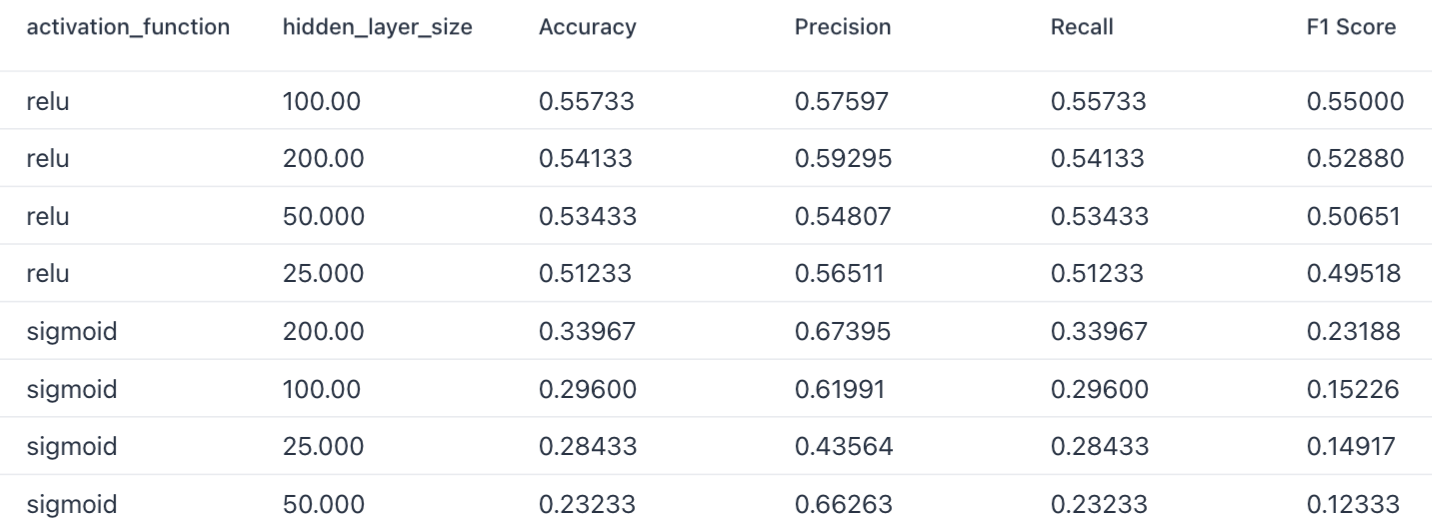
\includegraphics[width=1\linewidth]{images/FNN_tensorboard_table.png}
    \caption{Table containing the hyperparameters and the results of the hypertuning process performed.}
    \label{fig:FNN_table}
\end{figure}
The first model present in the image stands out as the best combination of tuned hyperparameters as it has the best results regarding the performance metrics. This model uses 100 neurons for each hidden layer, and a relu activation function in the three hidden layers. 

The best performance for relu is achieved with a hidden layer size of 100, with the following metrics:
\begin{itemize}
    \item Accuracy: 0.55733
    \item Precision: 0.57597
    \item Recall: 0.55733
    \item F1 Score: 0.55000
\end{itemize}

Sigmoid’s best performance is with a hidden layer size of 200, but its metrics are significantly lower:
\begin{itemize}
    \item Accuracy: 0.33967
    \item Precision: 0.67395
    \item Recall: 0.33967
    \item F1 Score: 0.23188
\end{itemize}

The relu activation function consistently outperforms sigmoid, even the best sigmoid model performs worse than any relu model. This is likely due to its ability to prevent vanishing gradient issues compared to sigmoid. When calculating the gradient for sigmoid its derivative is at most 0.25. The down side of this is when you have many layers the multiplication of these gradients tend to zero very quickly \cite{vanishing_grad}. 

The next figure provides a visual representation of the accuracy and loss trends for both training and validation data across the hyperparameter model over \textbf{30 epochs}, offering insights into the model's learning dynamics.

\begin{figure}[H]
    \centering
    \begin{subfigure}[t]{0.35\textwidth} % Tamanho de cada subfigura
        \centering
        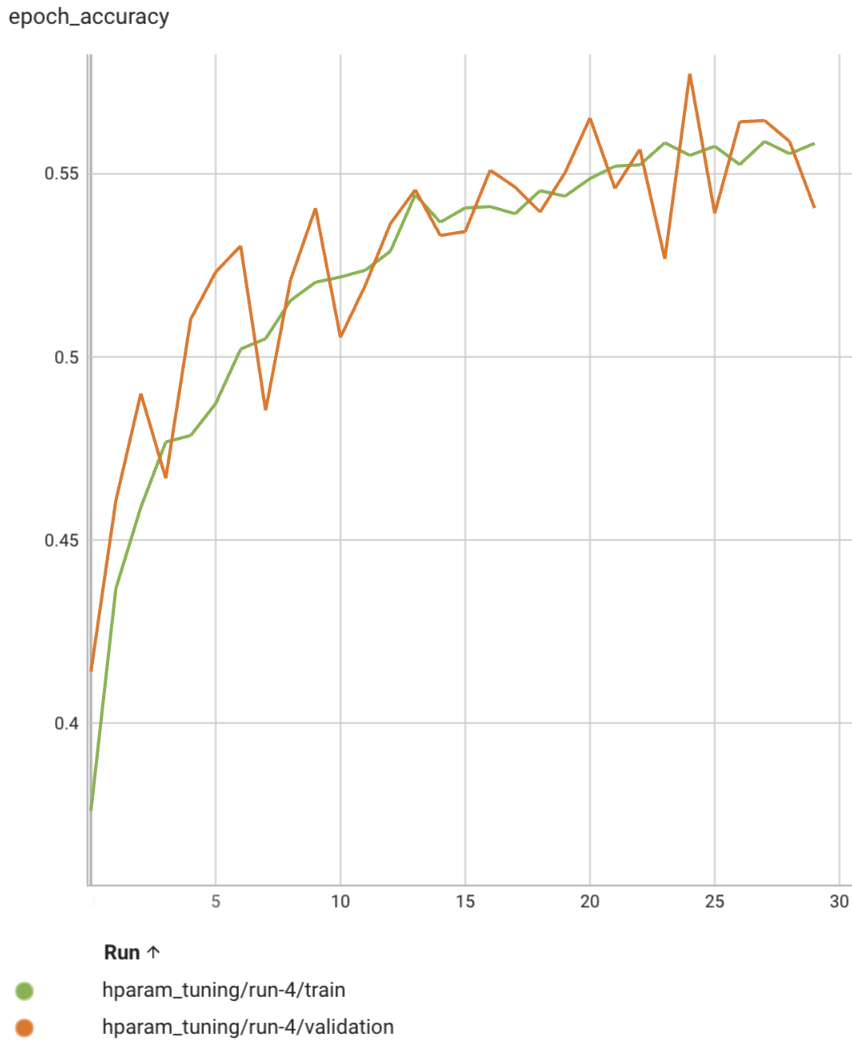
\includegraphics[width=\textwidth]{images/fnn_epoch_accuracy.png}
        \caption{Train vs Validation Accuracy over epochs}
        \label{fig:fnn_subfig1}
    \end{subfigure}
    \hfill
    \begin{subfigure}[t]{0.30\textwidth}
        \centering
        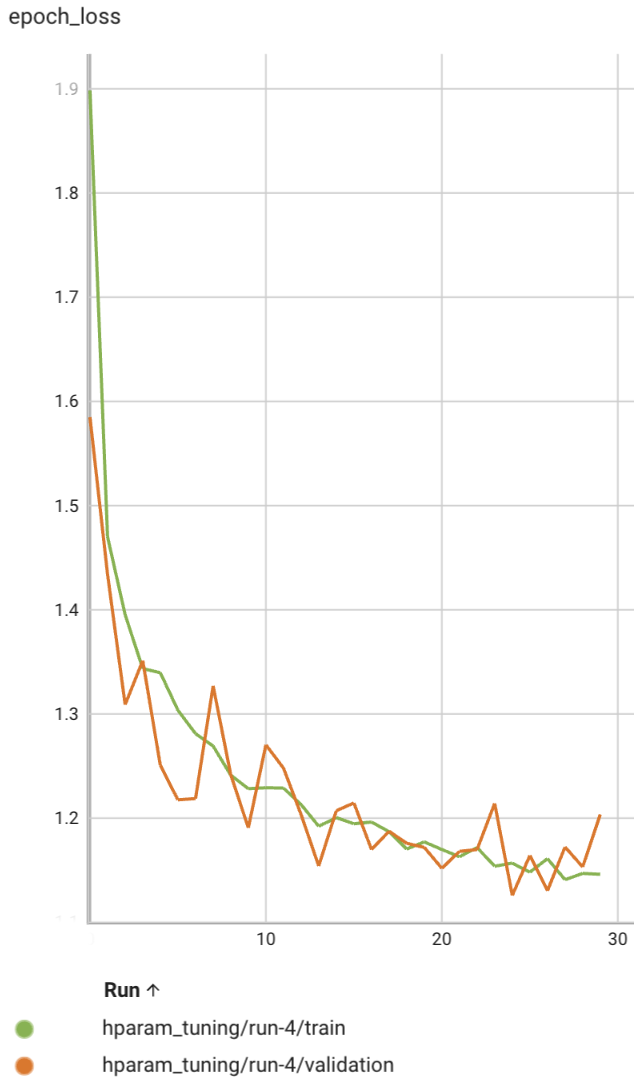
\includegraphics[width=\textwidth]{images/fnn_epoch_loss.png}
        \caption{Train vs Validation Loss over epochs}
        \label{fig:fnn_subfig2}
    \end{subfigure}
    \caption{Accuracy and Loss over epoch for the best set of hyperparameters FNN model.}
    \label{fig:images}
\end{figure}

As we can see in the first chart the training stabilizes by the 20th epoch, indicating that further training brings no significant improvements. The validation accuracy follows a similar trend to the training accuracy, increasing steadily during the early epochs. However, it also stabilizes after the 20th epoch. Both training and validation accuracies converge near the end of training. This suggests the model's performance on the validation set is close to that on the training set, suggesting good generalization. We can see there is little to no gap in both images between the training and validation curves which indicates the model does not overfit the training data.

To gain a deeper understanding of the model's performance, we can analyze the generated confusion matrix for the test data in the following image.
\begin{figure}[H]
    \centering
    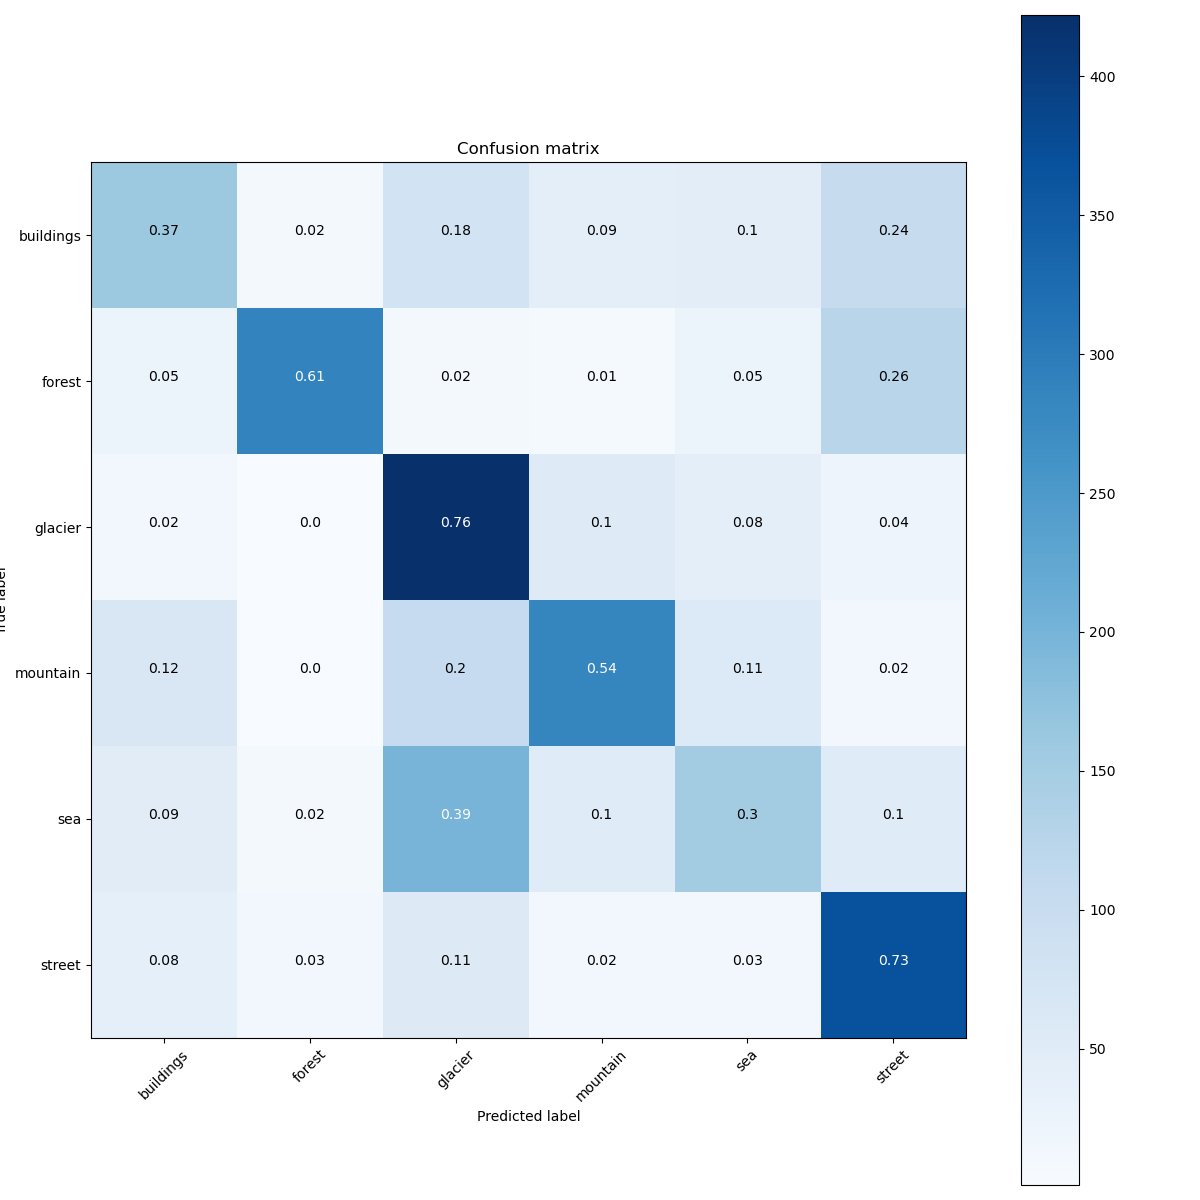
\includegraphics[width=1\linewidth]{images/fnn_cm.png}
    \caption{Confusion matrix of the best hyperparameter FNN model.}
    \label{fig:FNN_cm}
\end{figure}
This confusion matrix indicates the classes with the highest correct prediction rates are glacier and street, and the more challenging classes are buildings and sea. 

\subsection{Convolutional Neural Networks (CNNs)}
This CNNs approach uses a Data Augmentation training and validation set which is similar to the one used in the FNN approach described before.

The model architecture includes three convolutional layers, each followed by a max-pooling layer, with a fully connected dense layer and a dropout layer for regularization before the output layer. It is structured in the following table.

\begin{table}[H]
\centering
\caption{Architecture of the CNN Model}
\begin{tabular}{|l|}
\hline
\textbf{Layer (Type)}\\ \hline
Conv2D                      \\ \hline
MaxPooling2D                \\ \hline
Conv2D                      \\ \hline
MaxPooling2D                \\ \hline
Conv2D                      \\ \hline
MaxPooling2D                \\ \hline
Flatten                     \\ \hline
Dense                       \\ \hline
Dropout                     \\ \hline
Dense                  \\
\hline
\end{tabular}
\label{tab:cnn_architecture_2}
\end{table}

A grid search approach of hypertuning the model was used. It consisted of trying out different values of the hyperparameters and picking the "model" that gives the best score. This approach was used for balancing computational efficiency and thoroughness in exploring hyperparameter combinations. The hyperparameters that were tuned are the kernel/filter size, the dropout rate, and the optimizer function. The values experimented of each hyperparameter can be consulted in the table \ref{tab:cnn_hypertuning}.

\begin{table}[H]
\centering
\caption{CNN tuned hyperparameters.}
\begin{tabular}{|l|c|}
\hline
\textbf{Hyperparameter} & \textbf{Values} \\ \hline
Filter size & \{3, 5, 7\} \\ \hline
Dropout rate & \{0.2, 0.5\} \\ \hline
Otimizer & \{adam, sgd\} \\ \hline
\end{tabular}
\label{tab:cnn_hypertuning}
\end{table}

For each model created with a different set of hyperparameters the test confusion matrix and performance metrics were registered. This registration was made with the help of TensorBoard. Tensorboard is a python package that provides "visualization and tooling needed for machine learning experimentation"\cite{tensorboard}. It was instrumental in monitoring training and validation loss curves, ensuring proper convergence. The results for each model are kept in a logs folder which facilitates its detailed analysis.

In the image \ref{fig:CNN_table} all the performance metrics evaluated along with the tuned hyperparameters are exhibited.
\begin{figure}[H]
    \centering
    \includegraphics[width=1\linewidth]{images/CNN_tensorboard_table.png}
    \caption{Table containing the hyperparameters and the results of the hypertuning performed.}
    \label{fig:CNN_table}
\end{figure}
The first model present in the image stands out as the best combination of tuned hyperparameters as it has the best results regarding the performance metrics. It uses the adam optimizer, a kernel size of 3, and a dropout rate of 0.5. From the results we can understand that Adam consistently outperforms SGD. Smaller kernel sizes (3 or 5) generally perform better, with Adam paired with kernel size of 3 being the most effective.

The next figure provides a visual representation of the accuracy and loss trends for both training and validation data across the hyperparameter model over \textbf{30 epochs}, offering insights into the model's learning dynamics.

\begin{figure}[H]
    \centering
    \begin{subfigure}[t]{0.35\textwidth} % Tamanho de cada subfigura
        \centering
        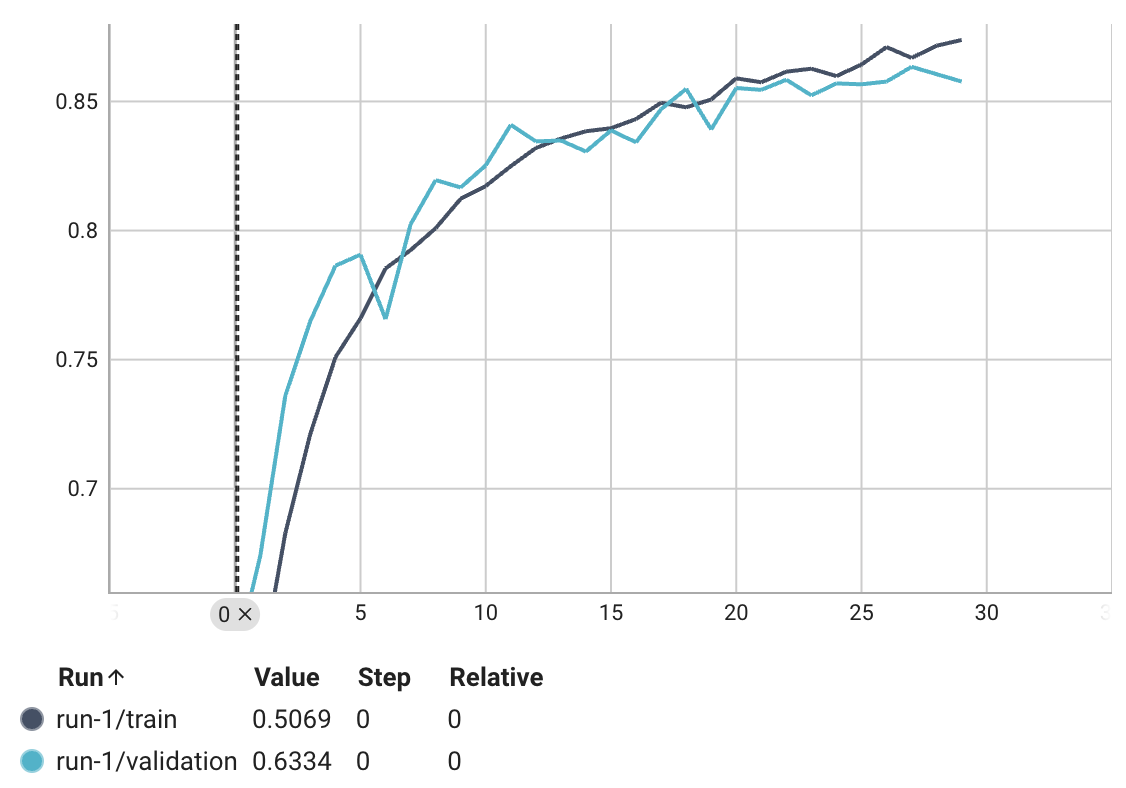
\includegraphics[width=\textwidth]{images/cnn_epoch_accuracy.png}
        \caption{Train vs Validation Accuracy over epochs}
        \label{fig:cnn_subfig1}
    \end{subfigure}
    \hfill
    \begin{subfigure}[t]{0.30\textwidth}
        \centering
        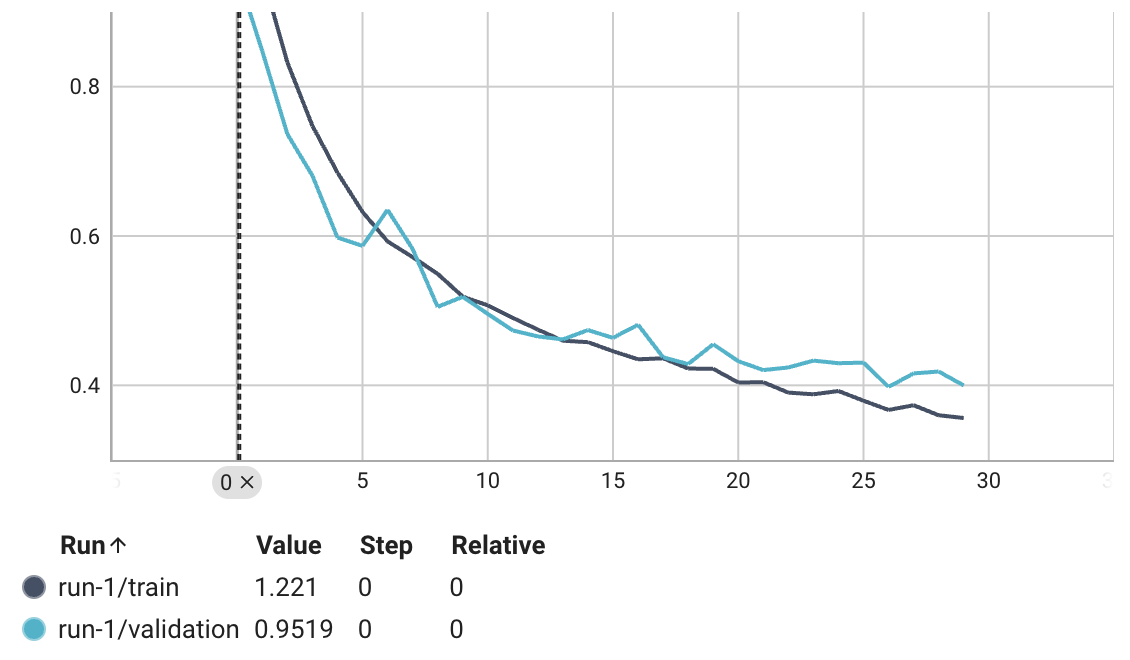
\includegraphics[width=\textwidth]{images/cnn_epoch_loss.png}
        \caption{Train vs Validation Loss over epochs}
        \label{fig:cnn_subfig2}
    \end{subfigure}
    \caption{Accuracy and Loss over epoch for the best set of hyperparameters CNN model.}
    \label{fig:images}
\end{figure}

As we can see in the first chart the training stabilizes by the 20th epoch, indicating that further training brings no significant improvements. The validation accuracy follows a similar trend to the training accuracy, increasing steadily during the early epochs. However, it also stabilizes after the 20th epoch. Both training and validation accuracies converge near the end of training. This suggests the model's performance on the validation set is close to that on the training set, suggesting good generalization. We can see there is little to no gap in both images between the training and validation curves which indicates the model does not overfit the training data.

To gain a deeper understanding of the model's performance, we can analyze the generated confusion matrix for the test data in the following image.
\begin{figure}[H]
    \centering
    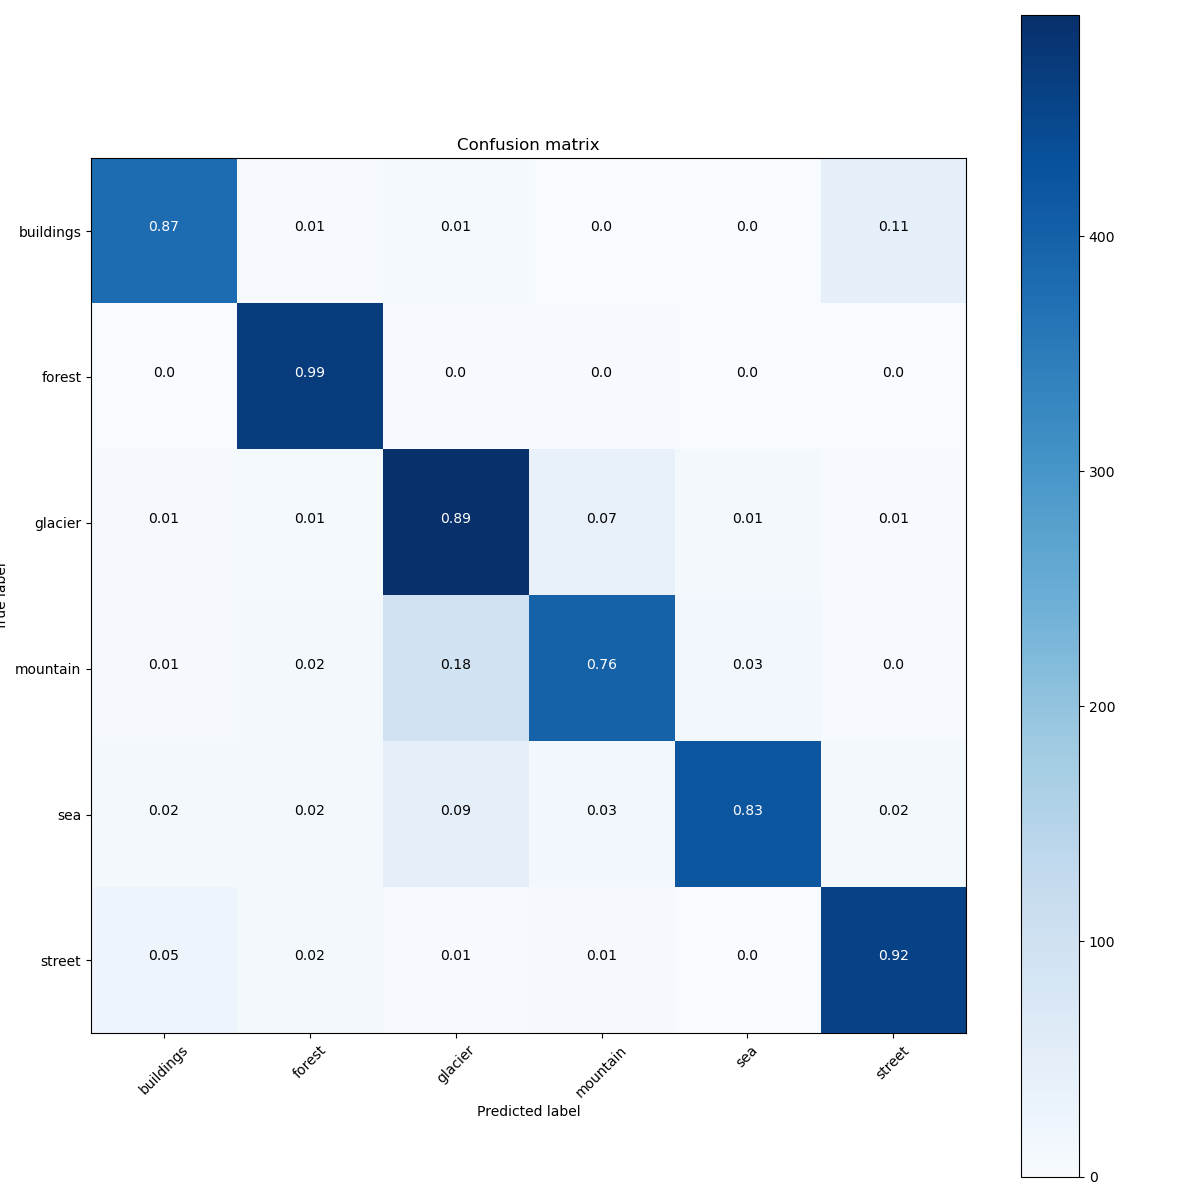
\includegraphics[width=1\linewidth]{images/cnn_tensorboard_cm.png}
    \caption{Confusion matrix of the best hyperparameter CNN model.}
    \label{fig:CNN_cm}
\end{figure}

The confusion matrix indicates the model performs exceptionally well on Forest and Street classes, suggesting strong feature extraction and learning for these categories. Overall there is minimal missclassifications which highlights the robustness of the model in distinguishing between classes.
The largest source of misclassification are mountains vs glaciers, 18\% of mountains are predicted as glaciers. This suggests overlapping features or insufficiently distinct feature extraction for these classes. The 11\% missclassification rate for buildings as streets show that urban environments are challenging to classify.